%!TEX program = pdflatex
\documentclass[masterarbeit,grey,german]{mas-thesis-chapters}				% Available options:
															% masterarbeit, bachelorarbeit, dissertation,
															% masterprojekt, bachelorprojekt, seminararbeit,
															% fallstudie, grey (für Graustufen), english


\usepackage{amsmath} % Mathematic Formulas
 \usepackage{acronym} % Acronyms


\usepackage{lmodern} % Latin Modern
 
% Create own Symbol Index
\newglossary[slg]{symbolslist}{syi}{syg}{Symbolverzeichnis}
 
% Disable Point at the end of Descriptions
\renewcommand*{\glspostdescription}{}
 
%Enable Glossar Commands
\makeglossaries
 
% Load Glossary File
\loadglsentries{chapters/Glossar}
 

\author{Michael Jokic}
\title{Analyse von Bandbreitenmessmethoden in mobilen Netzen}
\supervisor{Dr. Florian Metzger}	% ~ for nicer spaces
\reviewerA{Univ. Prof. Dr. Tobias Ho�feld}
\reviewerB{Univ. Prof. Dr. Jos\'{e} Marr\'{o}n}
\degreecourse{Angewandte Informatik - Systems Engineering}
\location{Essen}
%\linespread{1.25} % Line spread (default is 1.25)
\handoverdate{19.09.2016}

%%%%%%%%%%%%%% 
%TODO:

%\usepackage{array}


%% load bibs
\addbibresource{bibliography/bibliography.bib}
%\addbibresource{bibliography/more-bibliography.bib}

%\input{components/info}

%\DeclareBibliographyCategory{ownpub}

%%%%%%%%%%%%%%%%%%%%%%%%%%%%%%%%%%%%%%%%%%%%%%%%%%%%%%%%%%%%%%%%%%%%%%%%%%%%%%%%
\begin{document}

\maketitle			% Title Page

\pagenumbering{Roman}
\tableofcontents		% Table of Contents

\newpage

\listofillustrations	% List of Figures and List of Tables


\cleardoublepage

\pagenumbering{arabic}
\setcounter{page}{1}

\chapter{Introduction}	% Remove if not dissertation or masterarbeit

\section{Abstract}

This document is a short example of how to use this template to write your own thesis. It gives a brief summary of the most important aspects and options that define this template.

\newpage

\newpage
\section{Einleitung}

Die Bandbreite ist eine der wichtigsten Verbindungscharakteristiken zwischen zwei Hosts. Unter der Bandbreite wird in der Telekommunikation die tats�chlich �bertragene Datenmenge pro Zeiteinheit angegeben. Die kleinste Dateneinheit ist das Bit, weshalb die Bandbreite meist in Bit pro Sekunde (bit/s, b/s) oder einem Vielfachen davon angegeben wird.\cite{Bandbreite} Das Wissen �ber die aktuell verf�gbare Bandbreite ist gerade im mobilen Bereich interessant, da dort durch Funk�bertragung nicht immer ein stabiles Netz aufgrund von Umwelteinfl�ssen etc. garantiert werden kann.
\\
Durch den immer weiter fortschreitenden Ausbau des mobilen Netzes verschiebt sich die Nutzung des Internets immer mehr in diesen Bereich. So wird sich das Datenvolumen im mobilen Bereich in den n�chsten Jahren vervielfachen.\cite{Datenvolumen} Aus diesem Grund wird die verf�gbare Bandbreite zu einem immer entscheidenderen Faktor f�r Anwender und Anwendungen. Die wachsende Nutzung des mobilen Internets wird auch durch die wachsende Anzahl der Smartphone-Nutzer verst�rkt, welche in den  kommenden Jahren ebenfalls weiter steigt.\cite{SmartphoneUser}
\\\\
Durch die wachsende Smartphonenutzung ergeben sich auch neue M�glichkeiten zur Datensammlung und Auswertung. Da jedes Smartphone �ber eine Reihe von Sensoren verf�gt (Beispiel: GPS, Licht, Ger�usch) k�nnen diese Werte in Kombination verwendet werden um objektive Daten verschiedener Orte zu erfassen. Die so durchgef�hrte Datenerfassung kann durch Nutzung vieler unterschiedlicher Anwenderger�te viele Daten sammeln. Dies wird als Crowd Sensing bezeichent. Crowd Sensing ist das Sammeln von Daten durch gro�e Menschenmengen beziehungsweise durch deren mobile Endger�te. 
\\\\
In dieser Arbeit wird eine App f�r mobile Ger�te entwickelt, welche durch unterschiedliche Messverfahren die aktuelle Bandbreite ermittelt. Durch weitere Daten wie Orts- und Zeitinformationen k�nnen somit Aussagen �ber verf�gbare Bandbreiten getroffen werden.

\subsection{Motivation}

Das Wissen �ber die aktuell verf�gbare Bandbreite kann ein entscheidender Vorteil bei der Implementierung und Verwendung von Software sein. So kann auf Basis der verf�gbaren Bandbreite softwareseitig entschieden werden, ob Updates heruntergeladen werden sollen, oder ob dies auf einen sp�teren Zeitpunkt verschoben werden soll. Desweiteren kann softwareseitig bestimmt werden, in welchen Qualit�ten Videos wiedergegeben werden k�nnen. Dar�ber hinaus k�nnen Bandbreiten unterschiedlicher Schnittstellen gemessen werden und die f�r den jeweiligen Vorgang passende kann auf Grundlage dieser Ergebnisse ausgew�hlt werden.
\\\\
Die Bandbreite ist im Bereich der Mobilit�t ebenfalls ein entschiedender Faktor. Das Wissen �ber Bandbreiten an bestimmten Orten kann die Entscheidung eines Anwenders beeinflussen welche Aktivit�ten er im Internet verfolgt. Ob dieser nur einen Web-Artikel lesen oder aber einen Film in HD ansehen kann.
\\\\
Crowd Sensing ...

\subsection{Ziele}

Das Hauptziel dieser Arbeit ist die Analyse und der Vergleich unterschiedlicher Messmethoden zur Ermittlung der Bandbreite im mobilen Netz. Zu diesem Zweck ist es erforderlich, dass unterschiedliche Messmethoden betrachtet werden und f�r den Einsatz im mobilen Bereich untersucht und gegebenenfalls angepasst werden. Die entscheidenden Faktoren die die G�te der Messmethode beeinflussen sind prim�r die Genauigkeit, sowie das eingesetzte Datenvolumen, um eine Messung zu erhalten.
\\
F�r die eingesetzten Messmethoden m�ssen dar�ber hinaus Testabl�ufe entwickelt werden, unter der diese Methoden am effektivsten funktionieren. Die Effektivit�t bezieht sich hierbei wiederrum auf die Genauigkeit, sowie das Datenvolumen. Die daraus passenden Messmethoden werden f�r den Einsatz in einer App implementiert. Dar�ber hinaus wird f�r die App eine Anforderungsanalyse erstellt, welche zus�tzliche Funktionen und Einstellungsm�glichkeiten f�r die App definiert. Diese werden umgesetzt und getestet. 
\\\\
Mit der erstellten App werden �ber einen bestimmten Zeitraum Daten von erhoben. Diese werden analysiert und verglichen. Die Analyse umfasst dabei die Abdeckung der Bandbreite an unterschiedlichen Orten, sowie den Vergleich der eingesetzten Messmethoden. Der Vergleich bezieht sich auf unterschiedliche Faktoren der Messmethoden, wie zum Beispiel das ben�tigte Datenvolumen. Die gewonnenen Daten k�nnen zur Verdeutlichung der Ergebnisse dar�ber hinaus in einer Bandbreitenkarte dargestellt werden. Die Bandbreitenkarte kann somit Informationen zu verwendeten Providern oder auch der verf�gbaren Bandbreite an unterschiedlichen Orten dienen.

\newpage
\section{Verwandte Arbeiten}

Die Ermittlung der tats�chlich verf�gbaren Bandbreite ist ein wichtiger und interessanter Indikator von Internetverbindungen. Aus diesem Grund existieren eine Reihe von Arbeiten �ber Techniken zur Ermittlung der tats�chlichen Bandbreite. Die im Folgenden beschriebenen Arbeiten basieren alle auf unterschiedlichen Verfahren oder Berechnungen zur Ermittlung der verf�gbaren Bandbreite und geben so die Gesamtheit der unterschiedlichen Ans�tze zur Bandbreitenbestimmung wieder.
\\\\
\textbf{Nettimer}
\\
Die von Kevin Lai und Mary Baker entwickelte Software Nettimer misst die verf�gbare Bandbreite des Bottlenecks einer Verbindung anhand von gesendeten Paketpaaren und deren zeitlichen Differenzen beim Senden und Empfangen. Aufgrund der Tatsache, dass eine Messung schon mit zwei versendeten Paketpaaren gemacht werden kann, beschr�nkt sich diese Methode auf ein minimales Datenvolumen. \cite{Nettimer}
\\
\textbf{Pathload}
\\
Pathload ist eine von Manish Jain und Constantino Dovrolis entwickelte Software welche die Ende-zu-Ende verf�gbare Bandbreite einer Verbindung ermittelt. Patload basiert auf der Versendung von Paketz�gen. Diese Paketz�ge bestehen aus mehreren einzelnen Paketen welche in bestimmten Abst�nden verschickt werden. Anhand der Anpassung der zeitlichen Abst�nde kann die maximale Bandbreite ermittelt werden. \cite{Pathload}
\\
\textbf{PathChirp}
\\
PathChirp basiert �hnliche wie Pathload ebenfalls auf der Versendung von Paketz�gen. Anders als bei Pathload werden die Pakete des Paketzuges nicht mit konstantem Abstand versendet, sondern dieser Abstand wird mit fortlaufender Paketanzahl immer weiter verringert. Die Verringerung wird solange fortgesetzt, bis die maximale Bandbreite erreicht wird. Im Gegensatz zu Pathload hat PathChirp ein erheblich verringertes Datenvolumen. \cite{PathChirp}
\\
\textbf{STAB}
\\
STAB wurde unter anderem von Vinay J. Ribeiro entwickelt, welcher auch an PathChirp mitgewirkt hat. STAB ist eine Kombination aus Paketz�gen und der Versendung von kleinen und gro�en Paketen. Die Versendung von kleinen und gro�en Paketen geschieht aus dem Grund, dass kleine Pakete bei Ann�herung an die maximal verf�gbare Bandbreite noch beim Empf�nger ankommen, wohingegen gro�e Pakete verworfen werden. Aus den Ankunftszeiten der kleinen Pakete kann die Bandbreite ermittelt werden. \cite{STAB}
\\
\textbf{GPing}
\\
GPing wurde von Mingyang Zhong, Peizhao Hu und Jadwiga Indulska speziell zur Messung der Bandbreite in mobilen Netzen entwickelt, welches Limitierungen anderer Messmethoden minimieren soll. GPing basiert auf der Versendung von ICMP-Nachrichten und den daraus resultierenden Sende- und Ankunftszeiten dieser Nachrichten. \cite{GPing}
\\
\textbf{Spruce}
\\
Spruce ist ein von Jacob Strauss und Dina Katabi entwickeltes Programm welches �hnlich wie Nettimer auf der Versendung von Paketpaaren und deren Ankunftszeiten basiert. Dar�ber hinaus ben�tigt Spruce zur Berechnung der Bandbreite Informationen �ber die maximale Kapazit�t einer Verbindung. \cite{Spruce}
\\
\textbf{JPerf}
\\
JPerf ist ein in Java entwickeltes Programm mit grafischer Benutzeroberfl�che, welches auf dem Kommandzeilenprogramm iperf basiert. JPerf misst die Bandbreite anhand des Datendurchsatzes. Aus diesem Grund ben�tigt JPerf immer eine Client-Server-Architektur. Zwischen Client und Server werden Daten ausgetauscht und der Datendurchsatz wird anhand der Daten und der Dauer der �bertragung dieser Daten gemessen. \cite{JPerf}
\\
Mit Ausnahme von GPing welches Ping-Nachrichten auf Basis von ICMP-Nachrichten versendet, ben�tigen alle anderen Verfahren eine Client-Server-Architektur zur Messung von Paketzeiten. Die Messverfahren auf denen diese Programme basieren werden in dieser Arbeit teilweise verwendet.
Der Unterschied ist, dass diese Verfahren speziell in mobilen Netzwerken eingesetzt werden sollen und es daher erforderlich ist, dass sie in einer App umgesetzt werden. GPing ist die einzige beschriebene Methode, die sich ebenfalls mit der Thematik der Bandbreitenbestimmung in mobilen Netzen befasst.
Unterschiedliche Verfahren werden implementiert und werden daraufhin untereinander verglichen und bewertet.
\\
Neben unterschiedlichen Verfahren zur Ermittlung der Bandbreite existieren dar�ber hinaus auch eine Reihe von Apps die Bandbreitenmessungen durchf�hren. Als Beispiele sind hier Apps wie Speedtest.net\footnote[1]{\url{https://play.google.com/store/apps/details?id=org.zwanoo.android.speedtest&hl=de}} oder DSL Speedtest\footnote[2]{\url{https://play.google.com/store/apps/details?id=uk.co.broadbandspeedchecker}} zu nennen. Die Messungen dieser Apps zur Ermittlung der Download- und Upload-Bandbreite basieren allerdings auf dem tats�chlich erzielten Datendurchsatz durch das Verschicken von gr��eren Datenmengen. Dieses Datenvolumen soll durch die oben erw�hnten Methoden deutlich reduziert werden, sodass auch mit deutlich reduziertem Datenaustausch m�glichst genaue Ergebnisse erzielt werden.
\\\\
Ein weiteres Thema dieser Arbeit ist neben der Ermittlung der Bandbreite auch die Sammlung von Ger�tespezifischen Daten. Die Ermittlung der Bandbreite ist ohne zum Beispiel Orts- oder Zeitinformationen eher uninteressant. Im Bereich der Ger�te- oder Personenbezogenen Datensammlung existieren vor allem im mobilen Feld sehr viele Programme. Sensor Box for Android\footnote[3]{\url{http://downloadandroid.info/}} und AndroSensor\footnote[4]{\url{http://www.fivasim.com/androsensor.html}} sind zwei Beispiele f�r Apps welche Sensordaten  erheben. Die zur�ckgegebenen Werte der unterschiedlichen Sensoren eines Ger�tes wie zum Beispiel Lichtsensor oder auch Gyroskop k�nnen eingesehen und der zeitliche Verlauf der Werte betrachtet werden.
\\
Neben Apps zur Erhebung von Sensordaten existieren auch eine Reihe von Arbeiten zum Thema Datenerhebung und Datensammlung. In einem Versuch der UC Berkeley wurden GPS-Daten von Handys dazu verwendet, um Verkehrsdaten zu sammeln. Mit Hilfe der Daten konnten Reisezeiten und Geschwindigkeiten anhand einer bestimmten Route ermittelt werden. \cite{UCBTraffic}
In dieser Arbeit werden neben anderen Daten ebenfalls GPS-Daten erhoben. Die daraus resultierenden Ergebnisse k�nnen bei der Bestimmung von Bandbreiten an bestimmten Orten n�tzlich sein.
\\
Ein weiterer Artikel von Katie Shilton besch�ftigt sich mit der Frage der Privatsph�re bei der Sammlung von Daten einzelner Personen. In diesem Zusammenhang wird auch der Frage nachgegangen wie Daten generell gesch�tzt werden k�nnen und welche M�glichkeiten Anwendern von Entwicklerseite zum Schutz ihrer Daten einger�umt werden m�ssen. \cite{Privacy} Die in dieser Arbeit entwickelte Software besch�ftigt sich ebenfalls mit dem Thema des Datenschutzes, da neben der eigentlichen Bandbreitenmessung auch Informationen zu Ort und Zeit gesammelt werden.

% Erw�hnen, wie viel Datenvolumen jede Methode ben�tigt

% GPing als Packet Tailgating Methode als Variante von Packet Pair mit gro�em und kleinem Paket

\chapter{Messmethoden}

Es existieren unterschiedliche Methoden um die Bandbreite zu bestimmen. Ein Verfahren zur Bestimmung der Bandbreite ist der Download. Durch den Download einer entsprechend gro�en Datei kann der tats�chlich erreichte Datendurchsatz ermittelt werden. Diese Methode ist die genaueste, eignet sich allerdings nicht so gut, da zu viel Daten anfallen und es unter Umst�nden sehr lange dauern kann. Aus diesem Grunde werden im Folgenden Methoden vorgestellt, welche diese Probleme umgehen, und trotzdem die Bandbreite ermitteln k�nnen.
\\\\
Grob k�nnen diese Methoden in zwei Klassen eingeteilt werden. Die erste Klasse bestimmt die Bandbreite durch Verz�gerungszeiten einzelner versendeter Pakete, die durch weiteren Datenverkehr verursacht werden. Diese Klasse wird als Cross Traffic Estimation bezeichnet. Die zweite Klasse bestimmt Bandbreiten mittels �berlastung (Congestion) der Verbindung. Dabei wird die Bandbreite der maximalen Bandbreite bis zur �berlastung des Kanals schrittweise durch Versenden von Paketen angepasst. Diese Klasse wird als Self Induced Congestion bezeichnet.

%-----------------------------------------------------------------------------------------------------------------------------------------------------------------------------

\section{Cross Traffic Estimation}

Cross Traffic schickt Proben einzelner Pakete ins Netz und misst durch Verz�gerungen der Pakete die Bandbreite.
Cross Traffic interagiert mit weiterem Datenverkehr im Netz, der an einzelnen Routern anf�llt. Durch diesen Vorgang werden die versendeten Proben an Routern zwischengespeichert und es kommt zu Verz�gerungen.
In dieser Klasse gibt es zwei Ans�tze. Versendung eines einzelnen Paketes. Versenden von mehreren Paketen. Bei zwei Paketen gibt es noch eine Variante namens Packettailgating, bei der nicht zwei gleichgro�e Pakete, sondern ein kleines und ein gro�es Paket versendet werden.

%-----------------------------------------------------------------------------------------------------------------------------------------------------------------------------

\subsection{Paketumlaufzeit (Round Trip Time)}

Diese Methode entspricht in etwa dem Download, allerdings kann sie auch mit kleineren Datenmengen schon ziemlich genau den Datendurchsatz bestimmen. Unter der Round Trip Time (RTT) wird die Zeit verstanden, die ein Paket ben�tigt, um von einer Quelle zum Ziel und wieder zur�ck zu kommen. Dieses Konzept wird auf den Download einer kleineren Datenmenge angewendet. Zur Berechnung der Bandbreite wird eine kleine Datenmenge (ca. 0,5 MB) geladen und die Zeit zwischen Anfrage und Empfang der Datei gemessen. Die Bandbreite (B\textsubscript{RTT}) berechnet sich indem die Paketgr��e oder bezogene Datenmenge (P) durch die Paketumlaufzeit (RTT) geteilt wird.

\begin{align*}
B\textsubscript{RTT} =\frac { P} {RTT}
\end{align*}

%-----------------------------------------------------------------------------------------------------------------------------------------------------------------------------

\subsection{Packet Pair (PP)}

Bei der Paket Pair Methode werden zwei Pakete gleicher Gr��e von einer Quelle zum Ziel und wieder zur�ck gesendet. Die beim Absenden und Empfangen gemessenen Ankunftszeiten der Pakete dienen zur Berechnung der Zeitunterschiede $\Delta$t\textsubscript{out} beim Senden und $\Delta$t\textsubscript{in} beim Empfangen. 

\begin{figure}[htbp]
	\centering
		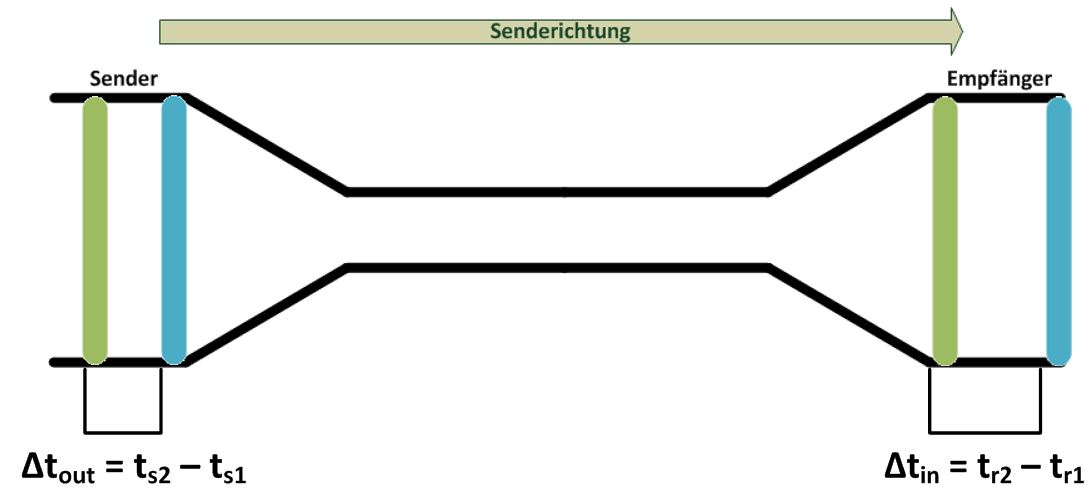
\includegraphics[scale=0.54]{images/PP.png}
		\caption{Schematischer Ablauf der Paket Pair Methode}
		\label{pp}
\end{figure}

In Abbildung \ref{pp} ist der Ablauf dieser Methode schematisch dargestellt. Die Abbildung zeigt eine Verbindung zwischen einem Sender und Empf�nger. Der schmale Teil der Verbindung stellt einen Bottleneck dar. Die beiden unterschiedlichen Pakete sind gr�n und blau gef�rbt. Vom Sender werden sie mit einer Zeitdifferenz von  $\Delta$t\textsubscript{out} losgeschickt. Mit diesem Abstand gelangen sie zum Bottleneck. Das blaue Paket wird durch den Bottleneck ohne Verz�gerung gesendet. Aufgrund von weiterem Datenverkehr auf dieser Leitung kann es vorkommen, dass das gr�ne Paket nicht direkt hinter dem blauen Paket gesendet wird. Es wird zwischengepuffert und die Zeit zwischen den Paketen vergr��ert sich. Durch diese auftretende Zeitdifferenz zwischen den Deltas kann eine Bandbreite berechnet werden. Zur Berechnung der Bandbreite (B\textsubscript{PP}) wird die Paketgr��e (P) eines Paketes durch die Differenz der beiden Deltas geteilt.\cite{Nettimer}

\begin{align*}
B\textsubscript{PP} = \frac { P}  {|(\Delta\textsubscript{in} - \Delta\textsubscript{out})|}
\end{align*}

%-----------------------------------------------------------------------------------------------------------------------------------------------------------------------------

\subsection{GPing}

GPing benutzt �hnlich wie die Paket Pair Methode zwei Pakete, welche hin und zur�ck gesendet werden um eine Bandbreite zu bestimmen. Bei GPing wird allerdings ein kleines Paket P\textsubscript{klein} mit wenigen Bytes (< 100) und ein gro�es Paket P\textsubscript{gro�} mit vielen Bytes (> 1000) versendet. Die RTT des kleinen Paketes RTT\textsubscript{klein} und die des gro�en Paketes RTT\textsubscript{gro�} werden separat voneinander bestimmt um so die Bandbreite zu berechnen.
Zur genaueren Messung werden mehrere Durchl�ufe n zur Bestimmung mehrerer RTTs gemacht. Die jeweils kleinste gemessene RTT pro Paket wird zur Berechnung der Bandbreite (B\textsubscript{GPing}) verwendet. Die zur Berechnung verwendeten RTTs werden zus�tzlich noch durch zwei geteilt, da nicht die komplette Verz�gerung, sondern nur die Einwegverz�gerung zur Berechnung ben�tigt wird.

\begin{align*}
B\textsubscript{GPing} = \frac {2 * (P\textsubscript{gro�} - P\textsubscript{klein})} {(min(RTT\textsubscript{gro�}) -  min(RTT\textsubscript{klein}))}
\end{align*}

%-----------------------------------------------------------------------------------------------------------------------------------------------------------------------------

\section{Self Induced Congestion}

Bei dieser Klasse wird die Bandbreite durch eine eigens erzeugte �berlastung des Netzwerkes berechnet. Dies wird erreicht, indem viele Pakete in kurzen Abst�nden hintereinander versendet werden, um das Netzwerk mit Paketen zu fluten. Die Last die dabei erzeugt wird erreicht somit nach Anpassung der Sendefrequenz irgendwann den Punkt, andem das Netz seine maximale Bandbreite erreicht.

%-----------------------------------------------------------------------------------------------------------------------------------------------------------------------------

\subsection{Packet Train (PT)}

Die Paket Train Methode basiert auf dem Versenden von Paketz�gen. Dabei besteht ein Paketzug aus mehreren Paketen der Anzahl n, welche in gleichem Abstand $\Delta$t voneinander versendet werden. Die Gr��e der Pakete ist P Bytes und ist f�r alle Pakete gleich. Die �bertragungszeit eines Paketes des Paketzuges betr�gt T. Der Abstand $\Delta$t zwischen den Paketen wird vom Sender an die gegebene Situation angepasst.
Aus diesen Werten kann der Sender eine �bertragungsrate R berechnen, mit der die Pakete versendet werden.

\begin{align*}
R\textsubscript{PT} = \frac {P} {T + \Delta t}
\end{align*}

Vor dem Versenden der Pakete wird jedes mit einem Zeitstempel t\textsubscript{i} versehen. Der Empf�nger berechnet nach Empfang der Pakete mit Hilfe der Ankunftszeit a\textsubscript{i} des jeweiligen Paketes die relative Verz�gerung D\textsubscript{i} = a\textsubscript{i} - t\textsubscript{i}. Wenn alle Verz�gerungswerte der Pakete berechnet wurden, werden diese miteinander verglichen, um festzustellen, ob die momentane Senderate R zur verf�gbaren Bandbreite B passt. 
Wenn die �bertragungsrate R gr��er als die aktuell verf�gbare Bandbreite ist, m�ssen die Pakete an einem entsprechenden Punkt der Verbindung zwischengepuffert werden, sodass die Verz�gerung des i-ten Paketes gr��er wird, als die des Paketes zuvor. Wenn nun R > A ist, so kann dies an den Verz�gerungswerten der Pakete gesehen werden, da diese mit steigender Anzahl der Pakete immer gr��er werden. Den umgekehrten Trend, wenn die Verz�gerungszeiten kleiner werden, sieht man, wenn R < A ist. 
\\
Durch diese Beobachtungen kann der Empf�nger dem Sender mitteilen, ob die aktuelle Senderate der Bandbreite entspricht, oder nicht.\cite{Pathload}

%-----------------------------------------------------------------------------------------------------------------------------------------------------------------------------

\section{Vergleich}

Die unterschiedlichen Messverfahren werden anhand der Daten die zeitgleich durch die Nutzung des Downloads berechnet wurden, verglichen. Da die Bandbreite durch den Download am exaktesten bestimmt werden kann, werden diese Daten als Richtlinie zum Vergleich genommen.
\\
Der Vergleich st�tzt sich im Detail auf zwei wichtige Kenngr��en. Zum einen ist dies das verwendete Datenvolumen pro Messung und zum anderen die Pr�zision der Messung. Weitere wichtige Faktoren sind die Messdauer pro Messung, sowie die Stabilit�t. Stabilit�t bezieht sich auf die Abweichungen der unterschiedlichen Messungen. Sind diese gering ist das Verfahren stabil, sind diese zwischen einzelnen Messungen in geringen Zeitabst�nden gro� ist das Verfahren eher instabil. Desweiteren wird auf Probleme bei den einzelnen Messmethoden eingegangen. 
\\\\
\textbf{RTT}
\\
Da RTT auf dem gleichen Prinzip wie der Download basiert, ist die Pr�zision ebenfalls ziemlich gut, bei signifikant kleinerem Datenverbrauch. Da pro Messdurchgang eine Datei mit fester Gr��e runtergeladen wird, kann der Datenverbrauch genau festgestellt werden. Um noch m�glichst pr�zise Bandbreiten du berechnen sollte die Datei nicht kleiner als 250 KB sein. Besser w�re noch 500 KB. Das Verfahren ist dar�ber hinaus relativ stabil und ben�tigt gegen�ber dem Download viel weniger Zeit.
\\\\
\textbf{PP}
\\
PP verschickt pro Messung nur zwei Pakete hat somit sehr wenig Datenverbrauch und die Messung kann schnell ausgef�hrt werden. Dadurch ist das Verfahren allerdings nicht sehr stabil und es m�ssen mehrere Messdurchg�nge durchgef�hrt werden, um aussagekr�ftige Ergebnisse zu bekommen. In kurzen Zeitabst�nden durchgef�hrte Messungen k�nnen daher sehr voneinander abweichen und somit ist die Pr�zision dieses Verfahrens mittelm��ig.
\\\\
\textbf{GPing}
\\
GPing verschickt wie PP ebenfalls nur zwei Pakete und hat somit ebenfalls wenig Datenverbrauch und eine geringe Messdauer. Das Verfahren liefert im Gegensatz zu PP allerdings wesentlich stabilere Werte, die bei aufeinander folgenden Messungen nur sehr wenig voneinander abweichen. Allerdings ist die Pr�zision dieser Methode sehr gering, da die Bandbreiten bei den durchgef�hrten Messungen immer 3 bis 4 Mal geringer waren, als die Vergleichswerte. 
\\\\
\textbf{PT}
\\
Da PT sich an die maximale Bandbreite durch verschicken von Paketz�gen heran tastet, schwankt der Datenverbrauch bei dieser Methode erheblich. Allerdings liegt dieser im Vergleich zum Download immer noch signifikant niedriger. Die Messdauer ist im Vergleich zum Download und RTT k�rzer, aber erheblich gr��er im Vergleich zu PP und GPing.

\begin{table}[H]
	\centering
		\begin{tabular}{|c|c|c|c|c|}
		\hline
			\textbf{Messverfahren} & \textbf{Pr�zision} & \textbf{Datenvolumen} & \textbf{Messdauer} & \textbf{Stabilit�t} \\
		\hline
			Download & Sehr hoch & 10 - 20 MB & Lang & Sehr hoch \\
		\hline
			RTT & Hoch & 250 KB (500 KB) & Mittel & Sehr hoch \\
		\hline
			PP & Mittel & 0,5 - 6 KB & Kurz & Gering \\
		\hline
			GPing & Gering & ca. 5 KB & Kurz & Sehr hoch \\
		\hline
			PT & Mittel & 100 - 500 KB & Lang & Mittel \\
		\hline
		\end{tabular}
	\caption{Vergleich der Messmethoden}
	\label{t-Comparison-Measurements}
\end{table}

%-----------------------------------------------------------------------------------------------------------------------------------------------------------------------------

\subsection{Probleme}

...
\newpage
\section{Umsetzung}

\subsection{Anforderungen}

\subsubsection{Messmethoden}

\subsubsection{App}

\subsection{Implementierung}
\chapter{Analyse}
\chapter{Ausblick}

...
\newpage
\section{Fazit}

\newpage

\printbibliography[heading=bibnumbered]

\glsaddall % print all Entries in Glossary even those without reference
% Print Glossary
\printglossary[style=altlist,title=Glossar]
 
% Print Acronyms
\deftranslation[to=German]{Acronyms}{Abk�rzungsverzeichnis}
\printglossary[type=\acronymtype,style=long,title=Abk�rzungsverzeichnis,toctitle=Abk�rzungsverzeichnis]
 
% Print Symbols
\printglossary[type=symbolslist,style=long]

\newpage

\makelicensepageCCBYSA

\end{document}
